\section{Introduction}
    
%%Due to the evolution of social media and mobile devices, massive network data is produced. 
%Distributed systems are at the core of the evolution of social media and mobile devices. This evolution leads to the creation of massive network data and efficient manipulation and usage of network data is becoming a major issue.  In order to process network data in parallel and perform tasks efficiently, many computing nodes are connected, providing users with services characterized by fault tolerance, ease of use and speed~\cite{tanenbaum}.
 
%Services running in distributed systems are difficult to be tested using traditional methods \cite{FaaS}. When faults occur in running services, faults can exponentially propagate \cite{verification_testing}. In this case, identifying faults in a running application in a production environment would go a long way. Testing in large scale distributed system is very hard due to the fact that the number of faults that can occur at any time is very large as well as it is very hard to imagine the scenarios that can accrue. Traditional testing techniques are not sufficient to predict the effects of faults on realistic applications running on large distributed systems \cite{FaaS}.
    
%Chaos Monkey, an open source project which adopts the fault injection technique, was developed by Netflix when they moved their data center to the cloud. The main function of Chaos Monkey is to inject random faults to the distributed system hosted on the cloud. While Chaos Monkey is used, fault injection is becoming a more popular technique for testing distributed systems, various researches on fault injection are springing out. At same time, other types of fault injection tools were also introduced, but most of them are used to test systems hosted on the cloud.     
    
As software for distributed systems becomes more complex, ensuring that a system meets its prescribed specification is a growing challenge for software developers~\cite{dawson1996testing}. Testing of large scale distributed systems may be very hard due to the fact that many different types of faults  can occur at any time  and it is very hard to imagine all possible scenarios that could occur as caused by interactions and collaborations among the distributed and potentially independent systems. 
%as well as it is very hard to imagine the scenarios that can occur. 
Traditional testing techniques are not sufficient to predict the effects of faults on real-world applications running on large distributed systems~\cite{FaaS}. In general, manual 
tests tend to test the existence of specified (known) failure modes, however, also %because of bugs in specification and code there are 
unknown failure modes  should be taken into account.

This is true in particular in testing system robustness, i.e. the degree to which a system can continue to function correctly even in the presence of invalid inputs or stressful environmental conditions~\cite{STANDARD}.
As a matter of facts, verifying the robustness of distributed system is not trivial. %Furthermore, the amount of faults that can occur is large. 
%Services running in distributed systems are difficult to be tested using traditional methods \cite{FaaS}. 
Moreover, when faults occur in running services, faults can exponentially propagate~\cite{verification_testing}. 
%Therefore, identifying faults in a running application in a production environment would go a long way. In particular, traditional testing will not provide a high confident testing level and it lacks of detecting unexpected faults. 
For this reason, testing should become % extended to testing executed at 
also a run-time activity~\cite{towards}. Online testing aims at evaluating systems in their real execution environment~\cite{Bertolino2012} and at validating %. 
%helps to detect the faults earlier, prevents faults from propagation and provides consistence tracing of faults. Testing at run-time can help to verify and validate 
that the system meets its requirements continuously. 
%\newline
%\pat{run-time testing or online testing?}

%In this paper we present a first step towards online testing. 
%The approach has been defined to capture faults before deploying to production. Chaos Monkey has been our inspiration, however the approach is not yet ready to be deployed on customers production networks. Instead the approach has been deployed on %internal 
%networks we run internally. %In other words, t
%Thanks to this approach we run the randomized tests in simulated environments and actual hardware but they are not part of a production environment.

In this paper we present an approach,  called \approach{}\footnote{\approach{} is a portmanteau fusing the word Postman and Monkey. The rational is that the approach is inspired by ChaosMonkey and applies it at the level of message exchange (content and delay) - this is why Postman.}, that has been conceived for online testing of system robustness for distributed embedded systems. \approach{} has been developed in collaboration with a team at Ericsson AB in Gothenburg, Sweden. % at Ericsson AB in Gothenburg. 
As said, when dealing with large scale distributed systems it is 
very hard to anticipate the possible scenarios that can occur as caused by interactions and collaborations among the distributed and potentially independent systems. This motivates the interest for robustness %that focuses on invalid inputs or stressful environmental conditions 
and for no-deterministic approaches that permit to go beyond specified and then known failure modes.

The \approach{}  approach provides non-deterministic testing method for checking the robustness of distributed embedded systems %. %The main idea is to check if the fault injection approach can be applicable to embedded distributed system. 
%Specifically we focus on systems consisting of small embedded components, 
with very limited computation power. \approach{} injects two different fault types, namely sending invalid messages and delaying the messages. We believe that randomized testing is a cost-effective way to complement traditional testing, remove potential  developer bias, and identify unknown failure modes. 

%The approach is called \approach{}\footnote{\approach{} is a portmanteau fusing the word Postman and Monkey. The rational is that the approach is inspired by ChaosMonkey and applies it at the level of message exchange (content and delay) - this is why Postman.}, and has been developed in collaboration with a team at Ericsson AB in Gothenburg, Sweden. 




%\approach{} injects two different fault types, namely sending invalid messages and delaying the messages. 
%This study is expected to benefits Ericsson who has an interest to test the robustness of their distributed system.
%The fault injection technique has been proposed as a possible way to address the fault tolerance challenges of distributed systems. This technique has been utilized for many years in order to verify the fault tolerance level of critical systems. Robustness of the system is important for Ericsson products and for embedded distributed systems. There is a need for Ericsson to have a fault injection tool in order to provide more robust products, the embedded industry is also calling for more research on utilizing fault injection on embedded distributed systems.
%\newline
%\section{Goals}
%The main purpose of this study is to test the robustness and availability of the distributed systems. In this thesis we present a fault injection approach that provides non-deterministic testing method for testing the robustness of the distributed systems. The main idea is to check if the fault injection approach can be applicable at Ericsson embedded distributed system. This study is expected to benefits Ericsson who has an interest to test the robustness of their distributed system.
%\newline 
%This work has been developed in collaboration with a team at Ericsson AB in Gothenburg, Sweden. % working on common subsystems for Radio Base Stations. % (called CNA). 
%Due to the complexity of distributed systems and the challenges of testing distributed systems with traditional approaches, a new approach based on some existing distributed systems testing technique and researches is needed. %The main investigation of this thesis is how to develop a new fault injection approach and implement a new fault injection tool to help the development team at Ericsson in testing their embedded distributed system. Moreover, we aim to make the fault injection approach as general as possible so it can be used in other companies and bring benefits to the embedded industry in general.
%\newline

%The fault injection approach and tool have been conceived and implemented in four iterations. 
%During the first iteration, we implemented the random messages sending, and during the second iteration we integrated the random messages sending into the automatic testing environment. Messages delaying was implemented during the third iteration and it was integrated into the automatic testing environment in the last iteration. 


%Each iteration was composed of four phases, namely: {\em Awareness of problem} %collecting information about different fault types through deep literature studying. By studying the previous related work, we took an inspiration for developing the new approach. Furthermore, 
%basically through %we had weekly 
%meetings with practitioners %the supervisors 
%at Ericsson and available documentation; %about the framework, 
%%organized by our industrial author 
%%in order to gather more information on how the system works as well as some suggestions about the injection. We also analyzed Ericsson PM framework documents for identifying the bottleneck of the system and determining the injections. Additionally, Ericsson's internal fault reports and other available documents helped in gathering more information about the weakness of the system and identifying where problems can occur. After deep studying of system weakness together with possible faults which might happen in reality, random faults were designed. At the same time the system was experimented by running with different scenarios and inspecting the log files. 
%%\item 
%{\em Suggestion and solution}, %Based on Ericsson fault report and designed fault tolerant ability of the PM framework, potential fault types were discussed with practitioners. We decided to have two fault types, the first one was sending random messages and the second one was delaying messages. In sending random messages, we got the idea from the supervisor in order to test the filter ability of the PM framework against random invalid messages. Delaying the messages were performed between the critical components of the PM framework where faults can occur.
%%\item 
%{\em Implementation}, and % The implementation contains two steps: tool development and tool integration. The first step mainly concerns the work of development the fault injection tool using an Ericsson internal shared library called Inter Process Communication. The second step mainly concerns the work of integrating the developed tool into the automatic testing environment of the PM framework.
%%\item 
%{\em Evaluation}. 
%




%The first step of the research has been collecting information about different fault types through deep literature studying. By studying the previous related work, we took an inspiration for developing the new approach. Furthermore, we had meetings with practitioners %the supervisors 
%at Ericsson organized by our industrial author in order to gather more information on how the system works as well as some suggestions about the injection. We also analyzed Ericsson PM framework documents for identifying the bottleneck of the system and determining the injections.
%%\newline

%Additionally, Ericsson's internal fault reports and other available documents helped in gathering more information about the weakness of the system and identifying where problems can occur. After deep studying of system weakness together with possible faults which might happen in reality, random faults were designed. At the same time the system was experimented by running with different scenarios and inspecting the log files. 

%Based on Ericsson fault report and designed fault tolerant ability of the PM framework, potential fault types were discussed with practitioners. We decided to have two fault types, the first one was sending random messages and the second one was delaying messages. In sending random messages, we got the idea from the supervisor in order to test the filter ability of the PM framework against random invalid messages. Delaying the messages were performed between the critical components of the PM framework where faults can occur.

%The implementation contains two steps: tool development and tool integration. The first step mainly concerns the work of development the fault injection tool using an Ericsson internal shared library called Inter Process Communication. The second step mainly concerns the work of integrating the developed tool into the automatic testing environment of the PM framework. 

%Evaluation is a very important phase in the development process. As a matter of fact, evaluation gives an indication of the conformance level of how the tool works. In this study tool evaluation included the following:   
%
%\begin{itemize}
%    \item Weekly meeting with the supervisor for getting feedback.
%    \item Well identified requirements for the expected conformance level on how the tool should work.
%    \item Continuous validation of the requirements.
%    \item Observing the results of running the fault injection tool through the log files.
%    \item Comparing the observed results with the expected (how the system should perform in its normal state). 
%    \item If faults were detected, evaluating the faults by tracing back to the cause that made them.
%\end{itemize}


%\newline

%Since 
To develop the approach, we followed an agile development process, and consequently \approach{} was evaluated continuously also through log files storing wanted and unwanted system behaviors, like system interrupts, messaging delaying, timeout and so on. Continuous evaluation of the approach helped us in developing the work as needed, decreasing the uncertainty level, and increasing the work quality. The source code of each iteration was pushed to a remote repository which practitioners had access to. During regular weekly meetings with practitioners, we got feedback on the fault injection approach and tool. Furthermore, during the last iteration we presented the fault injection approach and tool to the development team for a final validation.

%The faults caused by the new fault injection tool were monitored through log files, by analyzing the behaviors of the system through the log files, the new fault injection approach was evaluated continually. Everything appears in the log files introduced by the fault injection tool was analyzed in order to evaluate the tool. An example of unwanted system behavior can be like system interrupts, messaging delaying, timeout and so on.
%\newline

%Model evaluation mainly depended on the results of running the fault injection tool. If the PM framework crashes after running the fault injection tool, the actual injection and the reason of the crashing will be evaluated first. If the random message sending triggers the PM framework crashing, the message types, contents, amounts and the frequency of the sending will be evaluated first. Based on the expected fault tolerant ability of the PM framework and the possible fault types which might exist in reality, some unnecessary provoking will be filtered out. For example, sending random message A with content B triggered the system crashing, but in reality, message A can never contain content B, then we just filter such a random message away. If sending message A with content C triggered some bugs in the PM framework, and in reality message A might contain content C, then we keep such a random message. 
%%\newline
%
%The fault injection approach works based on random manner, random selection can be both realistic and not in its nature. In order to get a reasonable indication of the approach evaluation, we made the input selection of the tool less randomized. By doing so, the approach is evaluated in a reasonable way and the results helped in discovering the unexpected faults. As a result, evaluating the detected faults helped us in evaluating the internal code as well as system architecture. After that, some suggestions were proposed on how internal code and architecture can be improved.    

As a conclusion of this study, we show that fault injection techniques can be used for improving the robustness of embedded distributed
systems. Furthermore, using our approach we detected unexpected faults within distributed embedded systems of Ericsson. 
% where
%non deterministic testing is applied. 
Although the quality of system has been proven to be quite high, there have been some surprises, which were not caught by traditional testing: (i) fuzzing of signals has detected a weakness in handling dynamically sized objects causing a crash which then could be rectified, and (ii) randomized delays detected misconfigured timeout handling. It is important to highlight that the manual test case had the same mistake as the production code so the error was missed.

\approach{} also provided a clear indication of dependency bottlenecks, i.e. where faults might most probably occur. Consequently we could suggest improvements of the software architecture and some %keys of 
improvements
were built from the observed results. The approach is now adopted within the division of Ericsson with which we collaborated for realizing this work. 
%Finally, this approach came as a complementary
%of the existing traditional testing approach.
 At present stage, \approach{} has not yet been deployed in customer production networks, as further validation is ongoing. However, it is now used in networks that are run internally at Ericsson to capture faults at last stage before deployment to production. 
 
Summarizing, the main contribution of the paper is \approach{}, a non-deterministic testing approach for checking the robustness of distributed embedded systems with very limited computation power. The approach and lessons learned are general and can be adopted and replicated in other companies.
The successful collaboration model between academia and industry is based on iterative development/validation cycles and close collaboration with practitioners thus enabling continuous feedback and integration with real environments. 
%, and (ii)
%the successful collaboration model between academia and industry. Both contributions are general and can be adopted and replicated in other companies.

%\subsection{Paper structure}
This paper is structured as follows: Section~\ref{sec:context} identifies the context of the paper and presents the industrial environment in which we performed the research. Section~\ref{sec:relatedWorks} compares the approach to related works. Section~\ref{sec:researchMeth} presents the research methodology. Section~\ref{sec:approach} introduces  %the fault injection approach 
\approach{} and Section~\ref{sec:implementation} describes the implementation of the approach. Section~\ref{sec:results} reports the validation and results obtained by applying the approach on a real industrial environment. Section~\ref{sec:discussion} discusses lessons learned. Finally the paper concludes with final remarks and future research directions in Section~\ref{sec:conclusion}.

%\pat{add the structure} %section the structure of the report is specified. 

%\begin{description}
%  \item[Related Work] \hfill \\
%In the related work, we describe the previous related work. For each previous study we present the limitation, delimitation as well as the challenges that have been discovered on different literature study. Different concepts and terminology will be also presented for instance fault injection, failure as a service and the let it crash philosophy. Finally, we compare the previous related works with our thesis study. 
% 
%  \item[Research Approach] \hfill \\
%In the research approach section, we describe the research methodology used in this thesis Furthermore, we list the design and creation process starting from the awareness of the problem and ending with final conclusions. Additionally, we presents the implementation of the suggestion and solution. Finally, data gathering and analyzing were also described in this section.
%
%  \item[Results] \hfill \\
%In this section, the final results of running the fault injection approach are listed. Furthermore, from the extracted results an evident is drown on how well the fault injection approach work in this context. Finally, the tool is evaluated by comparing the results that we got with the previous techniques that Ericsson has.  
%  
%  \item[Discussion] \hfill \\
%In this section the results and the benefits of this study are discussed. Bottleneck of the system architecture will be also discussed. Moreover, key improvements of the architecture will be suggested.
%  
%  \item[Conclusion and future work] \hfill \\
%In this section, we list the final conclusion. Moreover, we present the lesson learned from this study. Finally, different aspects on how the work can be improved are suggested.
%\end{description}    
    
%\setcounter{page}{1}
%This chapter gives a brief introduction of fault injection and how it is currently used in the industry. Furthermore, the current problem that Ericsson has and the motivation of introducing a new fault injection technique are presented. This chapter ends with the goal of the thesis and the structure of the report.  

%\section{Background}
%Due to the evolution of social media and mobile devices, massive network data is produced. Distributed systems are at the core of this evolution. The need for efficient manipulation and usage of network data is a major issue.  In order to process network data in parallel and perform tasks efficiently, many computing nodes are connected, providing users with services characterized by fault tolerance, ease of use and speed \cite{tanenbaum}.
%\newline

\section{Context}\label{sec:context}

The usage of the Internet is continuously growing in the industry due to the fact that more and more devices are connected, as shown in Figure~\ref{ericsson_report}.
Specifically,  Machine-to-Machine (M2M) is expected to grow strongly, driven by new use cases, e.g., in
cars, machines and utility metering.  
 %As a result, more faults are introduced to the systems, and the systems are more likely to be affected by those faults. For this reason, d
Distributed systems need to be increasingly resilient to different types of faults and combinations of them as part of the system's normal operating procedure. Combination of faults may have a major impact on the performance of the system, sometimes even leading to systems being temporarily out of service, which has dramatic effects of embedded distributed systems, because such systems are increasingly fragile and safety critical~\cite{combination}. Distributed systems tend to have more unexpected faults than other types of systems when used in reality~\cite{FaaS}.
%\newline

\begin{figure}[h]
\centering
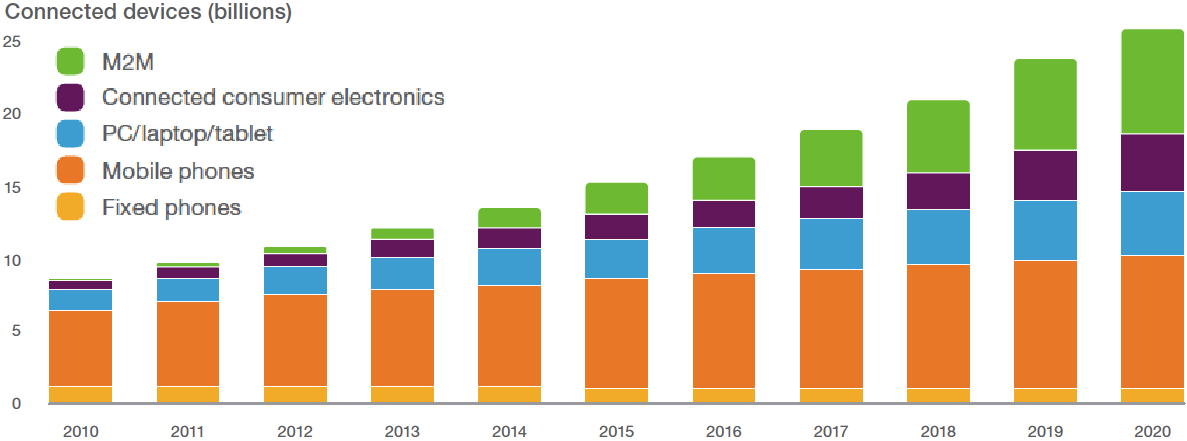
\includegraphics[width=\columnwidth]{figure/connected_devices.png}
\caption{Ericsson Mobility Report June 2015 \cite{connected_deveices} \label{ericsson_report}}
\end{figure}


%\section{Problem description}
RBS (Radio Base Station) is an integral part of the mobile data solutions delivered by Ericsson. A RBS consists of embedded components that are connected together in order to support high network availability to wide area network. A mobile network is a distributed system that consists of many RBSs. 
%Due to the fact that operators as well as subscribers expect that network services support almost everything in their daily life, so high availability of network services is an essential part in daily life. 
As long as network signalling volumes increase and operators demand more complex configurations for supporting more usage scenarios, the need for improving resilience is also increasing. The network should be flexible so that it responses to the challenge of the dramatic increasing in the network traffic and signaling created by the operators and subscribers~\cite{availability}.
%\newline

The Performance Management (PM) framework, one key component of RBS, is a framework used to count phone calls and network usages of subscribers. 
%Similarly to other components of RBS, the PM framework is tested using traditional approaches like unit testing and functional testing. % (mock testing~\cite{Mackinnon2001}). %; in this way %such 
%%software testing techniques are deterministic~\cite{deterministic}. 
%Unit testing %will not catch all errors in the code, since it cannot evaluate every execution path of the program. Unit testing 
%only tests the functionality of the units themselves, it will not catch integration or system-level errors. Although functional testing combines different test cases and tests the code at the system level, such a combination is usually limited. In fact, functional and unit testing approaches are deterministic~\cite{deterministic} and unknown failure modes % then random faults 
%are very hard to be detected. 
%%Therefore, there is a need of implementing a non-deterministic approach, fault injection approach uses random mechanism for detecting the unexpected faults at the same time can be utilized in large scale systems. So fault injection approaches can be complementary to the existing testing techniques. 
%%\newline
The RBS components, including the PM framework, are tested using traditional  approaches  like unit testing and functional testing.  Unit  testing  is the most adequate approach to test the functionality of the units taken individually, however it will not catch integration or system-level errors. Functional testing combines different test cases and can test the code at system level, however such a combination is usually limited. In fact, functional and unit testing approaches are deterministic and as such they mostly address failure modes that are expected. Potential unknown failure modes are very hard to be detected by traditional testing.

In order to catch also unknown failure modes, %do testing in a non-deterministic way,  
testing should be randomized and fault injection~\cite{nondeterministic} can be a valuable technique to be exploited for this purpose. 
While several approaches exist for fault injection, such as the already cited Chaos Monkey, they were not adequate for testing distributed embedded systems with very limited computational power such as the PM framework. This motivated the design and implementation of \approach{}. 
%which is specifically tailored for system with these characteristics: 
%%Some projects like Chaos Monkey use fault injection for online testing, but they were developed for testing distributed systems hosted on the cloud. Chaos Monkey is an open source project that has been developed by Netflix when they moved their data center to the cloud. The main function of Chaos Monkey is to inject random faults to the distributed system hosted on the cloud. 
%%%Fault injection is a popular technique for testing distributed systems, various researches on fault injection are springing out. At same time, other types of fault injection tools were also introduced, but most of them are used to test systems hosted on the cloud.  
%%RBS is a type of distributed system which consists of small embedded components. Previous approaches like Chaos Monkey are not feasible for such an embedded distributed system. Additional unavoidable requirements emerge for this type of systems, for instance: 
%limited computation and hardware capabilities, 
%%The new fault injection tool for such an embedded distributed system has new requirements; for instance the injection in the new fault technique is done 
%the fault injection must be done near to the hardware layer, %the programming language will be c++ instead of Java. On the other side, 
%the  fault injection technique must use shared libraries, %. Moreover, 
%the communication paradigm between the components should be inter-process communication.


%Each iteration was composed of four phases, namely:
%
%\begin{itemize}
%\item {\em Awareness of problem:} %collecting information about different fault types through deep literature studying. By studying the previous related work, we took an inspiration for developing the new approach. Furthermore, 
%we had weekly meetings with practitioners %the supervisors 
%at Ericsson organized by our industrial author in order to gather more information on how the system works as well as some suggestions about the injection. We also analyzed Ericsson PM framework documents for identifying the bottleneck of the system and determining the injections. Additionally, Ericsson's internal fault reports and other available documents helped in gathering more information about the weakness of the system and identifying where problems can occur. After deep studying of system weakness together with possible faults which might happen in reality, random faults were designed. At the same time the system was experimented by running with different scenarios and inspecting the log files. 
%\item {\em Suggestion and solution:} Based on Ericsson fault report and designed fault tolerant ability of the PM framework, potential fault types were discussed with practitioners. We decided to have two fault types, the first one was sending random messages and the second one was delaying messages. In sending random messages, we got the idea from the supervisor in order to test the filter ability of the PM framework against random invalid messages. Delaying the messages were performed between the critical components of the PM framework where faults can occur.
%\item {\em Implementation:} The implementation contains two steps: tool development and tool integration. The first step mainly concerns the work of development the fault injection tool using an Ericsson internal shared library called Inter Process Communication. The second step mainly concerns the work of integrating the developed tool into the automatic testing environment of the PM framework.
%\item {\em Evaluation:} 
%%Since we utilized agile development process, the fault injection approach was evaluated continually. Continuous evaluation of the approach helped us in developing the work as needed, decrease the uncertainty level, and increase the work quality. The source code of each iteration was pushed to the remote repository where the supervisor had access to it. During the weekly meeting with practitioners, we got feedback on the fault injection tool. Furthermore, we presented the fault injection tool after the last iteration to the development team and got some feedback from them. 
%\end{itemize}


%\section{Motivation}
%Services running in distributed systems are difficult to be tested using traditional methods \cite{FaaS}. When faults occur in running services, faults can exponentially propagate \cite{verification_testing}. In this case, identifying faults in a running application in a production environment would go a long way. Testing in large scale distributed system is very hard due to the fact that the number of faults that can occur at any time is very large as well as it is very hard to imagine the scenarios that can accrue. Traditional testing techniques are not sufficient to predict the effects of faults on realistic applications running on large distributed systems \cite{FaaS}.
%\newline


